% Options for packages loaded elsewhere
\PassOptionsToPackage{unicode}{hyperref}
\PassOptionsToPackage{hyphens}{url}
\PassOptionsToPackage{dvipsnames,svgnames,x11names}{xcolor}
%
\documentclass[
  letterpaper,
  DIV=11,
  numbers=noendperiod]{scrartcl}

\usepackage{amsmath,amssymb}
\usepackage{iftex}
\ifPDFTeX
  \usepackage[T1]{fontenc}
  \usepackage[utf8]{inputenc}
  \usepackage{textcomp} % provide euro and other symbols
\else % if luatex or xetex
  \usepackage{unicode-math}
  \defaultfontfeatures{Scale=MatchLowercase}
  \defaultfontfeatures[\rmfamily]{Ligatures=TeX,Scale=1}
\fi
\usepackage{lmodern}
\ifPDFTeX\else  
    % xetex/luatex font selection
\fi
% Use upquote if available, for straight quotes in verbatim environments
\IfFileExists{upquote.sty}{\usepackage{upquote}}{}
\IfFileExists{microtype.sty}{% use microtype if available
  \usepackage[]{microtype}
  \UseMicrotypeSet[protrusion]{basicmath} % disable protrusion for tt fonts
}{}
\makeatletter
\@ifundefined{KOMAClassName}{% if non-KOMA class
  \IfFileExists{parskip.sty}{%
    \usepackage{parskip}
  }{% else
    \setlength{\parindent}{0pt}
    \setlength{\parskip}{6pt plus 2pt minus 1pt}}
}{% if KOMA class
  \KOMAoptions{parskip=half}}
\makeatother
\usepackage{xcolor}
\setlength{\emergencystretch}{3em} % prevent overfull lines
\setcounter{secnumdepth}{5}
% Make \paragraph and \subparagraph free-standing
\makeatletter
\ifx\paragraph\undefined\else
  \let\oldparagraph\paragraph
  \renewcommand{\paragraph}{
    \@ifstar
      \xxxParagraphStar
      \xxxParagraphNoStar
  }
  \newcommand{\xxxParagraphStar}[1]{\oldparagraph*{#1}\mbox{}}
  \newcommand{\xxxParagraphNoStar}[1]{\oldparagraph{#1}\mbox{}}
\fi
\ifx\subparagraph\undefined\else
  \let\oldsubparagraph\subparagraph
  \renewcommand{\subparagraph}{
    \@ifstar
      \xxxSubParagraphStar
      \xxxSubParagraphNoStar
  }
  \newcommand{\xxxSubParagraphStar}[1]{\oldsubparagraph*{#1}\mbox{}}
  \newcommand{\xxxSubParagraphNoStar}[1]{\oldsubparagraph{#1}\mbox{}}
\fi
\makeatother


\providecommand{\tightlist}{%
  \setlength{\itemsep}{0pt}\setlength{\parskip}{0pt}}\usepackage{longtable,booktabs,array}
\usepackage{calc} % for calculating minipage widths
% Correct order of tables after \paragraph or \subparagraph
\usepackage{etoolbox}
\makeatletter
\patchcmd\longtable{\par}{\if@noskipsec\mbox{}\fi\par}{}{}
\makeatother
% Allow footnotes in longtable head/foot
\IfFileExists{footnotehyper.sty}{\usepackage{footnotehyper}}{\usepackage{footnote}}
\makesavenoteenv{longtable}
\usepackage{graphicx}
\makeatletter
\def\maxwidth{\ifdim\Gin@nat@width>\linewidth\linewidth\else\Gin@nat@width\fi}
\def\maxheight{\ifdim\Gin@nat@height>\textheight\textheight\else\Gin@nat@height\fi}
\makeatother
% Scale images if necessary, so that they will not overflow the page
% margins by default, and it is still possible to overwrite the defaults
% using explicit options in \includegraphics[width, height, ...]{}
\setkeys{Gin}{width=\maxwidth,height=\maxheight,keepaspectratio}
% Set default figure placement to htbp
\makeatletter
\def\fps@figure{htbp}
\makeatother

\usepackage{booktabs}
\usepackage{caption}
\usepackage{longtable}
\usepackage{colortbl}
\usepackage{array}
\usepackage{anyfontsize}
\usepackage{multirow}
\KOMAoption{captions}{tableheading}
\makeatletter
\@ifpackageloaded{caption}{}{\usepackage{caption}}
\AtBeginDocument{%
\ifdefined\contentsname
  \renewcommand*\contentsname{Table of contents}
\else
  \newcommand\contentsname{Table of contents}
\fi
\ifdefined\listfigurename
  \renewcommand*\listfigurename{List of Figures}
\else
  \newcommand\listfigurename{List of Figures}
\fi
\ifdefined\listtablename
  \renewcommand*\listtablename{List of Tables}
\else
  \newcommand\listtablename{List of Tables}
\fi
\ifdefined\figurename
  \renewcommand*\figurename{Figure}
\else
  \newcommand\figurename{Figure}
\fi
\ifdefined\tablename
  \renewcommand*\tablename{Table}
\else
  \newcommand\tablename{Table}
\fi
}
\@ifpackageloaded{float}{}{\usepackage{float}}
\floatstyle{ruled}
\@ifundefined{c@chapter}{\newfloat{codelisting}{h}{lop}}{\newfloat{codelisting}{h}{lop}[chapter]}
\floatname{codelisting}{Listing}
\newcommand*\listoflistings{\listof{codelisting}{List of Listings}}
\makeatother
\makeatletter
\makeatother
\makeatletter
\@ifpackageloaded{caption}{}{\usepackage{caption}}
\@ifpackageloaded{subcaption}{}{\usepackage{subcaption}}
\makeatother

\ifLuaTeX
  \usepackage{selnolig}  % disable illegal ligatures
\fi
\usepackage{bookmark}

\IfFileExists{xurl.sty}{\usepackage{xurl}}{} % add URL line breaks if available
\urlstyle{same} % disable monospaced font for URLs
\hypersetup{
  pdftitle={¿Qué justifica la violencia interétnica? Dinámicas entre indígenas y no indígenas en Chile desde un enfoque longitudinal (2016 - 2023)},
  pdfauthor={Matías Deneken; Ana Figuerido; Roberto González; Monica Gerber; Roberto Cantillán; Federico Díaz},
  colorlinks=true,
  linkcolor={blue},
  filecolor={Maroon},
  citecolor={Blue},
  urlcolor={Blue},
  pdfcreator={LaTeX via pandoc}}


\title{¿Qué justifica la violencia interétnica? Dinámicas entre
indígenas y no indígenas en Chile desde un enfoque longitudinal (2016 -
2023)}
\author{Matías Deneken \and Ana Figuerido \and Roberto
González \and Monica Gerber \and Roberto Cantillán \and Federico Díaz}
\date{}

\begin{document}
\maketitle

\renewcommand*\contentsname{Table of contents}
{
\hypersetup{linkcolor=}
\setcounter{tocdepth}{3}
\tableofcontents
}

\section{Abstract}\label{abstract}

(Escribir más adelante.)

\textbf{Keywords:} conflicto interétnico, violencia intergrupal,
legitimidad, justicia procedimental, Chile, análisis de clases latentes.

\section{1. Introducción}\label{introducciuxf3n}

\emph{Responsable: Matías Deneken}

(Plantear pregunta central, contribución, relevancia empírica y
teórica.)

El estudio del conflicto entre el Estado chileno y los pueblos
indígenas---especialmente el pueblo mapuche---ha estado marcado por
tensiones históricas, desigualdades estructurales y episodios
recurrentes de violencia intergrupal. Sin embargo, existe limitada
evidencia longitudinal sobre cómo cambian las actitudes hacia la
violencia interétnica y qué factores sociales y psicológicos legitiman
su uso. Este artículo aborda estas brechas mediante un diseño de clases
latentes aplicado a cuatro olas de la Encuesta Longitudinal de
Relaciones Interculturales (ELRI, 2016--2023).

\section{2. Perspectiva teórica}\label{perspectiva-teuxf3rica}

\subsection{2.1. El conflicto indígena en
Chile}\label{el-conflicto-induxedgena-en-chile}

(Repaso histórico y político hasta el proceso constituyente.)

\subsection{2.2. Relaciones intergrupales: contacto, confianza y
legitimidad}\label{relaciones-intergrupales-contacto-confianza-y-legitimidad}

(Enfocar en teorías de relaciones intergrupales, contacto, amenaza,
confianza social.)

\subsection{2.3. Justicia procedimental y violencia
intergrupal}\label{justicia-procedimental-y-violencia-intergrupal}

(Relacionar legitimidad institucional con apoyo a la violencia entre
grupos.)

\section{3. Métodos}\label{muxe9todos}

\subsection{3.1. Datos}\label{datos}

Utilizamos la \textbf{Encuesta Longitudinal de Relaciones
Interculturales (ELRI)}, un panel que sigue a personas indígenas y no
indígenas entre 2016 y 2023.

\subsection{3.2. Variables}\label{variables}

\subsubsection{3.2.1. Variable independiente
principal}\label{variable-independiente-principal}

Clases latentes construidas a partir de cuatro indicadores:

\begin{itemize}
\tightlist
\item
  Dos ítems asociados a \textbf{cambio social}.\\
\item
  Dos ítems asociados a \textbf{control social}.
\end{itemize}

\subsubsection{3.2.2. Variables
dependientes}\label{variables-dependientes}

Cada modelo incluye como desenlaces:

\begin{itemize}
\tightlist
\item
  Percepción de conflicto Estado--Pueblos Originarios\\
\item
  Confianza en pueblos originarios\\
\item
  Justicia procedimental hacia pueblos indígenas\\
\item
  Identificación con la causa indígena\\
\item
  Frecuencia de contacto\\
\item
  Urbano/rural\\
\item
  Mujer\\
\item
  Identidad indígena (indi / no indi)\\
\item
  Edad
\end{itemize}

(Se pueden agregar descriptivos en tabla.)

\subsection{3.3. Técnica analítica}\label{tuxe9cnica-analuxedtica}

Se estimaron \textbf{modelos de clases latentes (Latent Class Analysis,
LCA)} para identificar perfiles de legitimación de la violencia
interétnica. Posteriormente, se modeló la probabilidad de pertenencia a
cada clase como función de las variables dependientes mediante regresión
logística multinomial o transición latente (dependiendo del diseño
final).

\subsubsection{3.X. Modelo estructural}\label{x.-modelo-estructural}

\paragraph{3.X.1 Distribución inicial de las clases
latentes}\label{x.1-distribuciuxf3n-inicial-de-las-clases-latentes}

Sea (U\_\{it\} \in \{1,\dots,K\}) la clase latente del individuo (i) en
el tiempo (t), y (\mathbf{X}\_i) un vector de covariables individuales
(por ejemplo, edad, género, identidad indígena, zona urbana/rural,
confianza en pueblos originarios, percepción de conflicto, justicia
procedimental e identificación con la causa indígena).

La distribución inicial de las clases, en (t = 1), se modela mediante
una regresión logística multinomial:

\[
P(U_{i1} = u \mid \mathbf{X}_i) \;=\; 
\frac{\exp\big(\alpha_u + \mathbf{X}_i^\top \boldsymbol{\beta}_u\big)}
     {\displaystyle \sum_{v=1}^{K} \exp\big(\alpha_v + \mathbf{X}_i^\top \boldsymbol{\beta}_v\big)},
\quad u = 1,\dots,K,
\]

donde (\alpha\_u) es el intercepto específico de la clase (u) y
(\boldsymbol{\beta}\_u) es el vector de coeficientes asociado a las
covariables (\mathbf{X}\_i) para dicha clase. Una de las clases se toma
como referencia para asegurar la identificación del modelo.

\paragraph{3.X.2 Modelo de transición entre
clases}\label{x.2-modelo-de-transiciuxf3n-entre-clases}

Para estudiar la dinámica de las clases entre dos olas consecutivas,
modelamos la probabilidad de transición desde una clase de origen (v) en
(t-1) hacia una clase de destino (u) en (t), en función de las mismas
covariables (\mathbf{X}\_i). La estructura de transición se especifica
también mediante un modelo logístico multinomial:

\[
P\big(U_{it} = u \mid U_{i,t-1} = v,\; \mathbf{X}_i\big)
\;=\;
\frac{\exp\big(\gamma_{vu} + \mathbf{X}_i^\top \boldsymbol{\delta}_{vu}\big)}
     {\displaystyle \sum_{w=1}^{K} \exp\big(\gamma_{vw} + \mathbf{X}_i^\top \boldsymbol{\delta}_{vw}\big)},
\quad u = 1,\dots,K,
\]

donde (\gamma\emph{\{vu\}) es el intercepto de la transición desde la
clase (v) hacia la clase (u), y (\boldsymbol{\delta}}\{vu\}) recoge el
efecto de las covariables sobre dicha transición. En la práctica,
estimamos razones de odds (odds ratios) para comparar la probabilidad de
permanecer en la clase de referencia frente a la probabilidad de
transitar a las otras clases, en función de las variables de contacto,
confianza, percepción de conflicto, justicia procedimental,
identificación con la causa indígena y características
sociodemográficas.

\section{4. Resultados}\label{resultados}

Descriptivos

\begin{center}
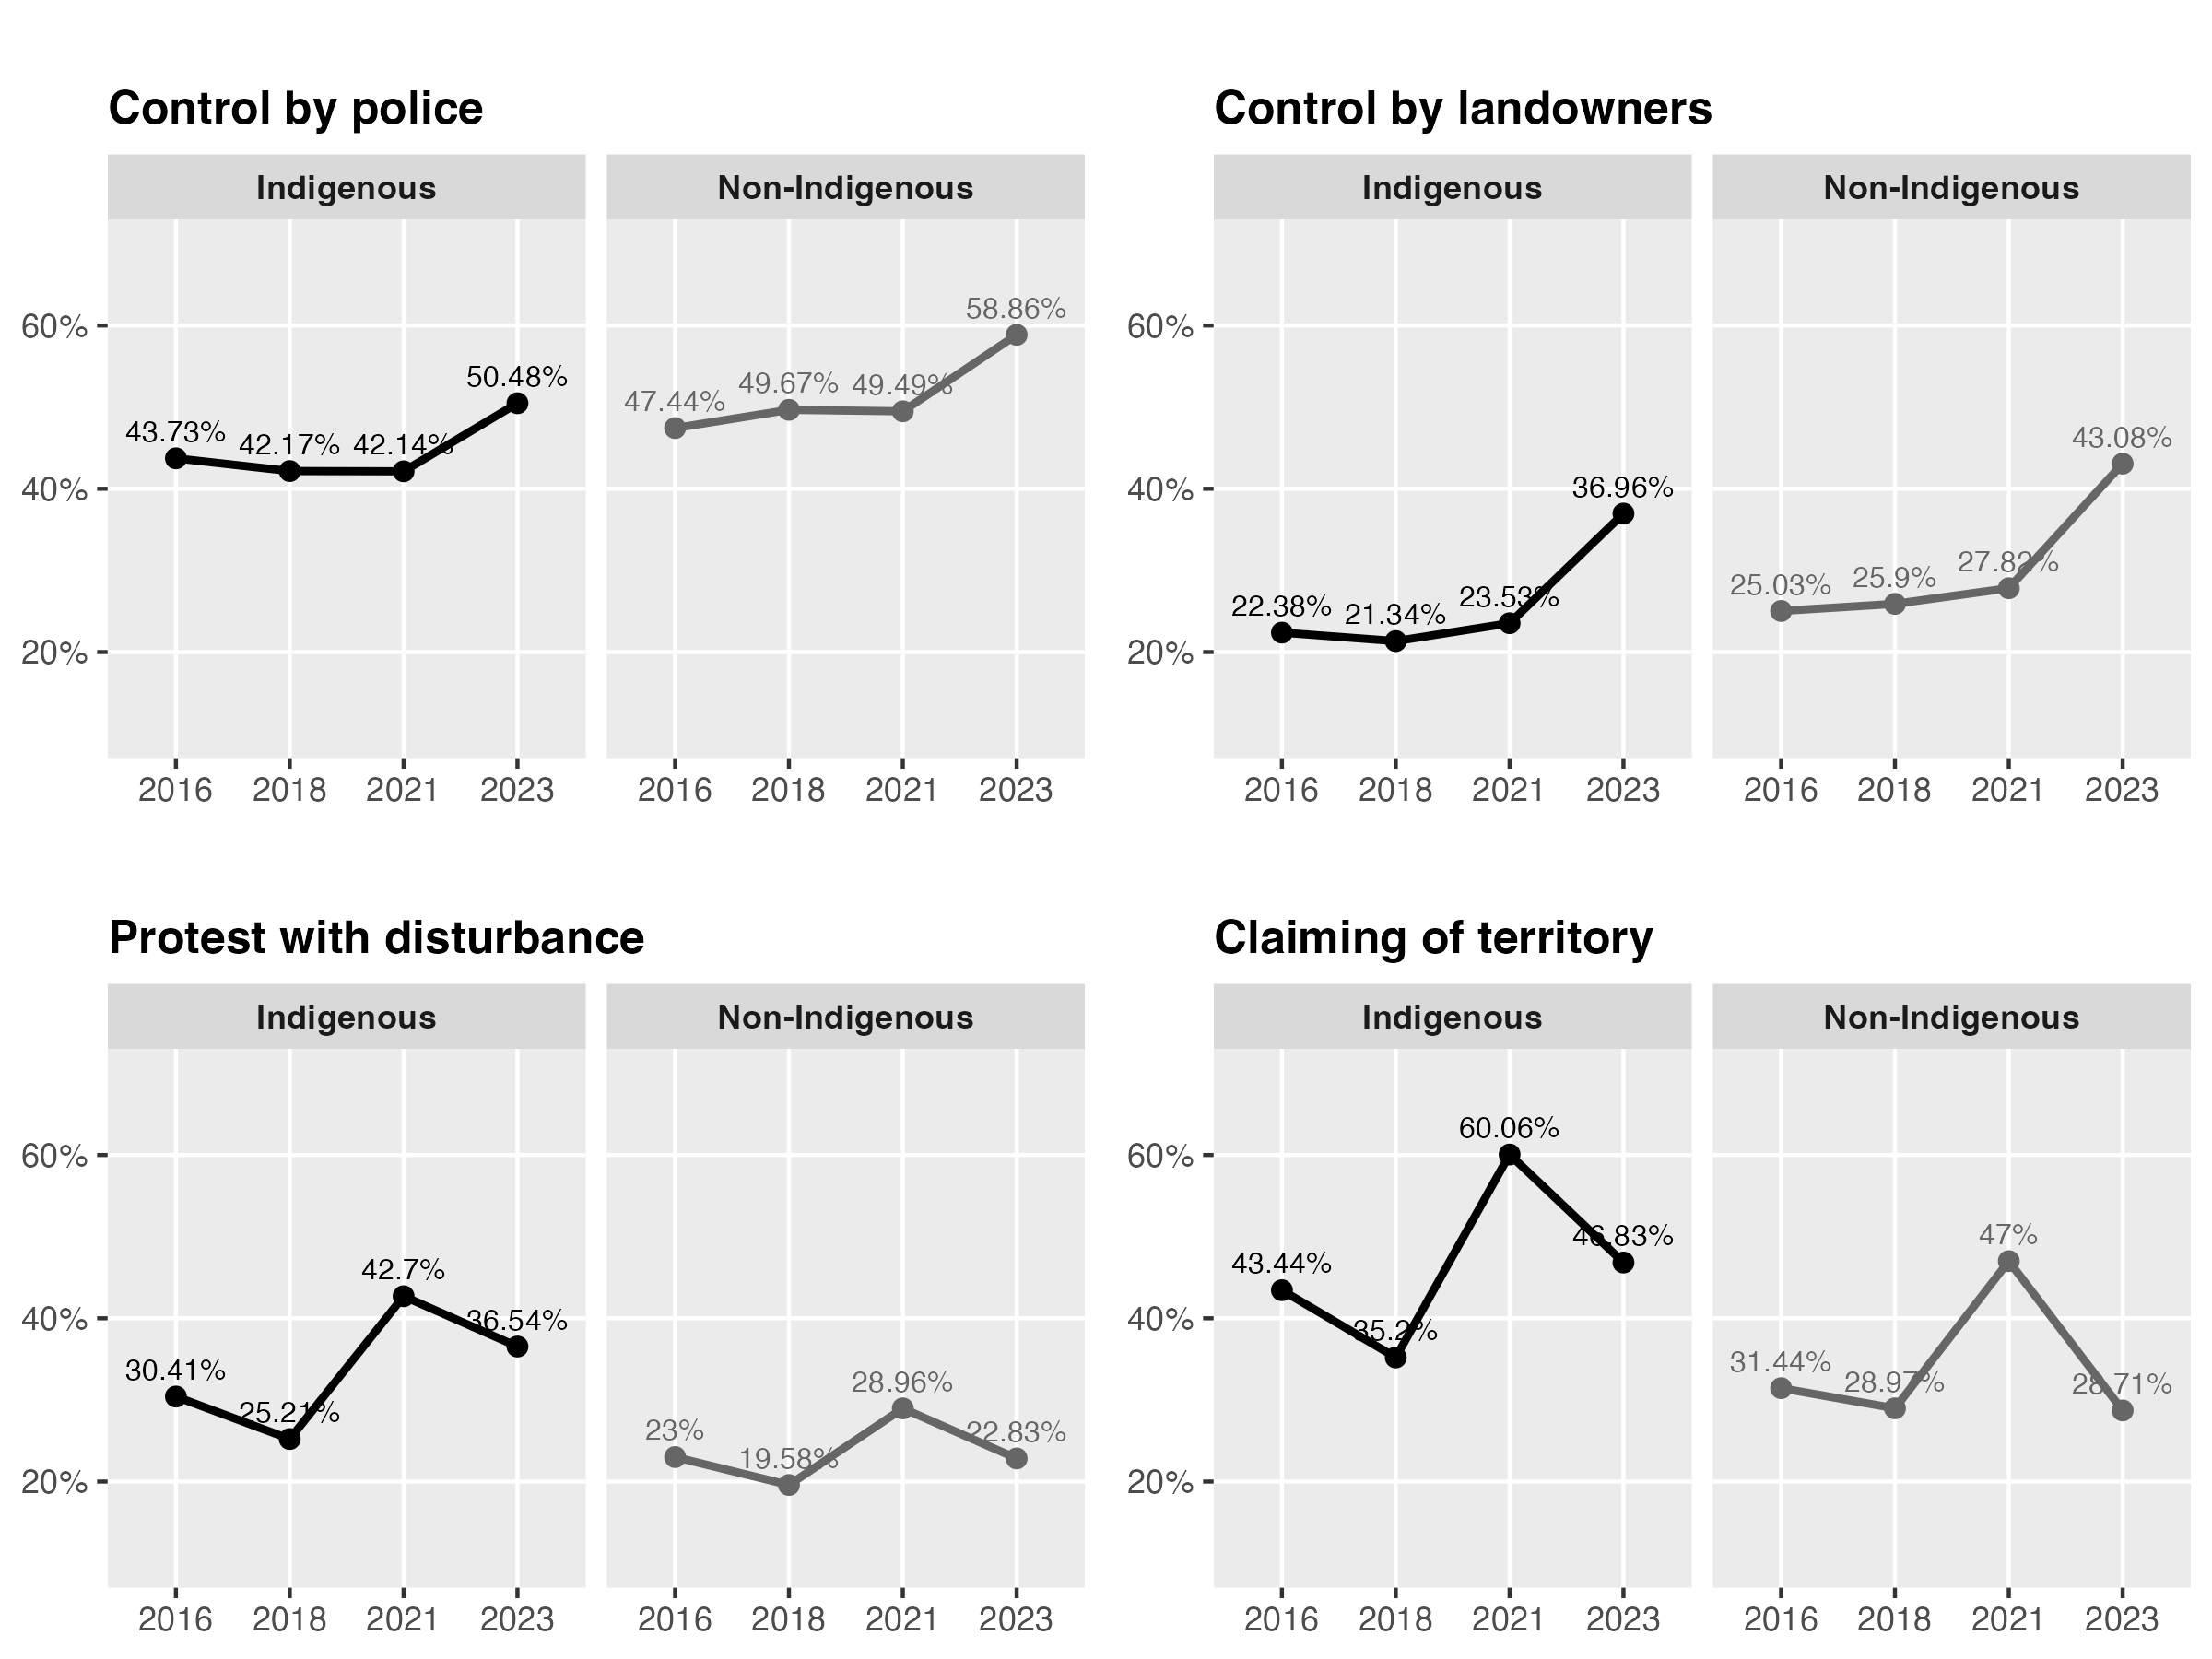
\includegraphics[width=4.1875in,height=\textheight]{images/justification_police_violence_indigenous-01.png}
\end{center}

\textbf{Primer resultado:} Clases y estabilidad de las mismas.

\begin{center}
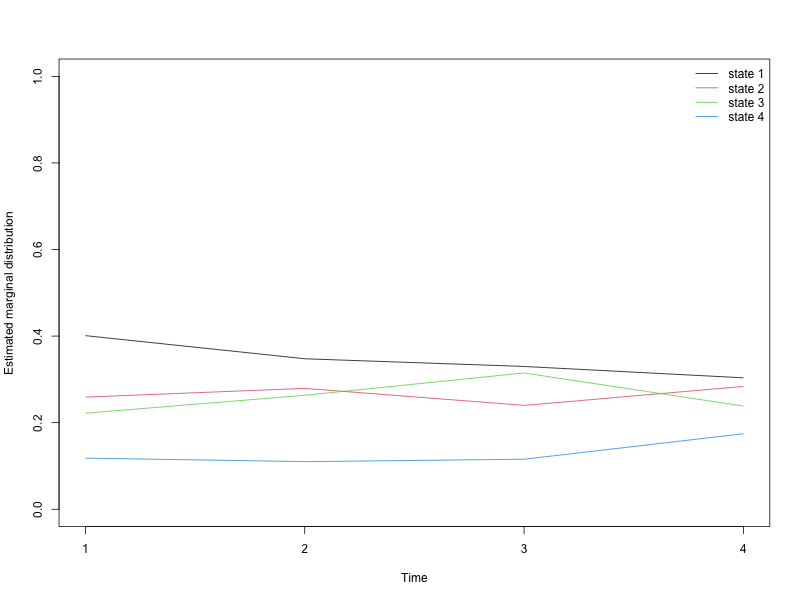
\includegraphics{images/marginal_distribution-01.png}
\end{center}

\begin{center}
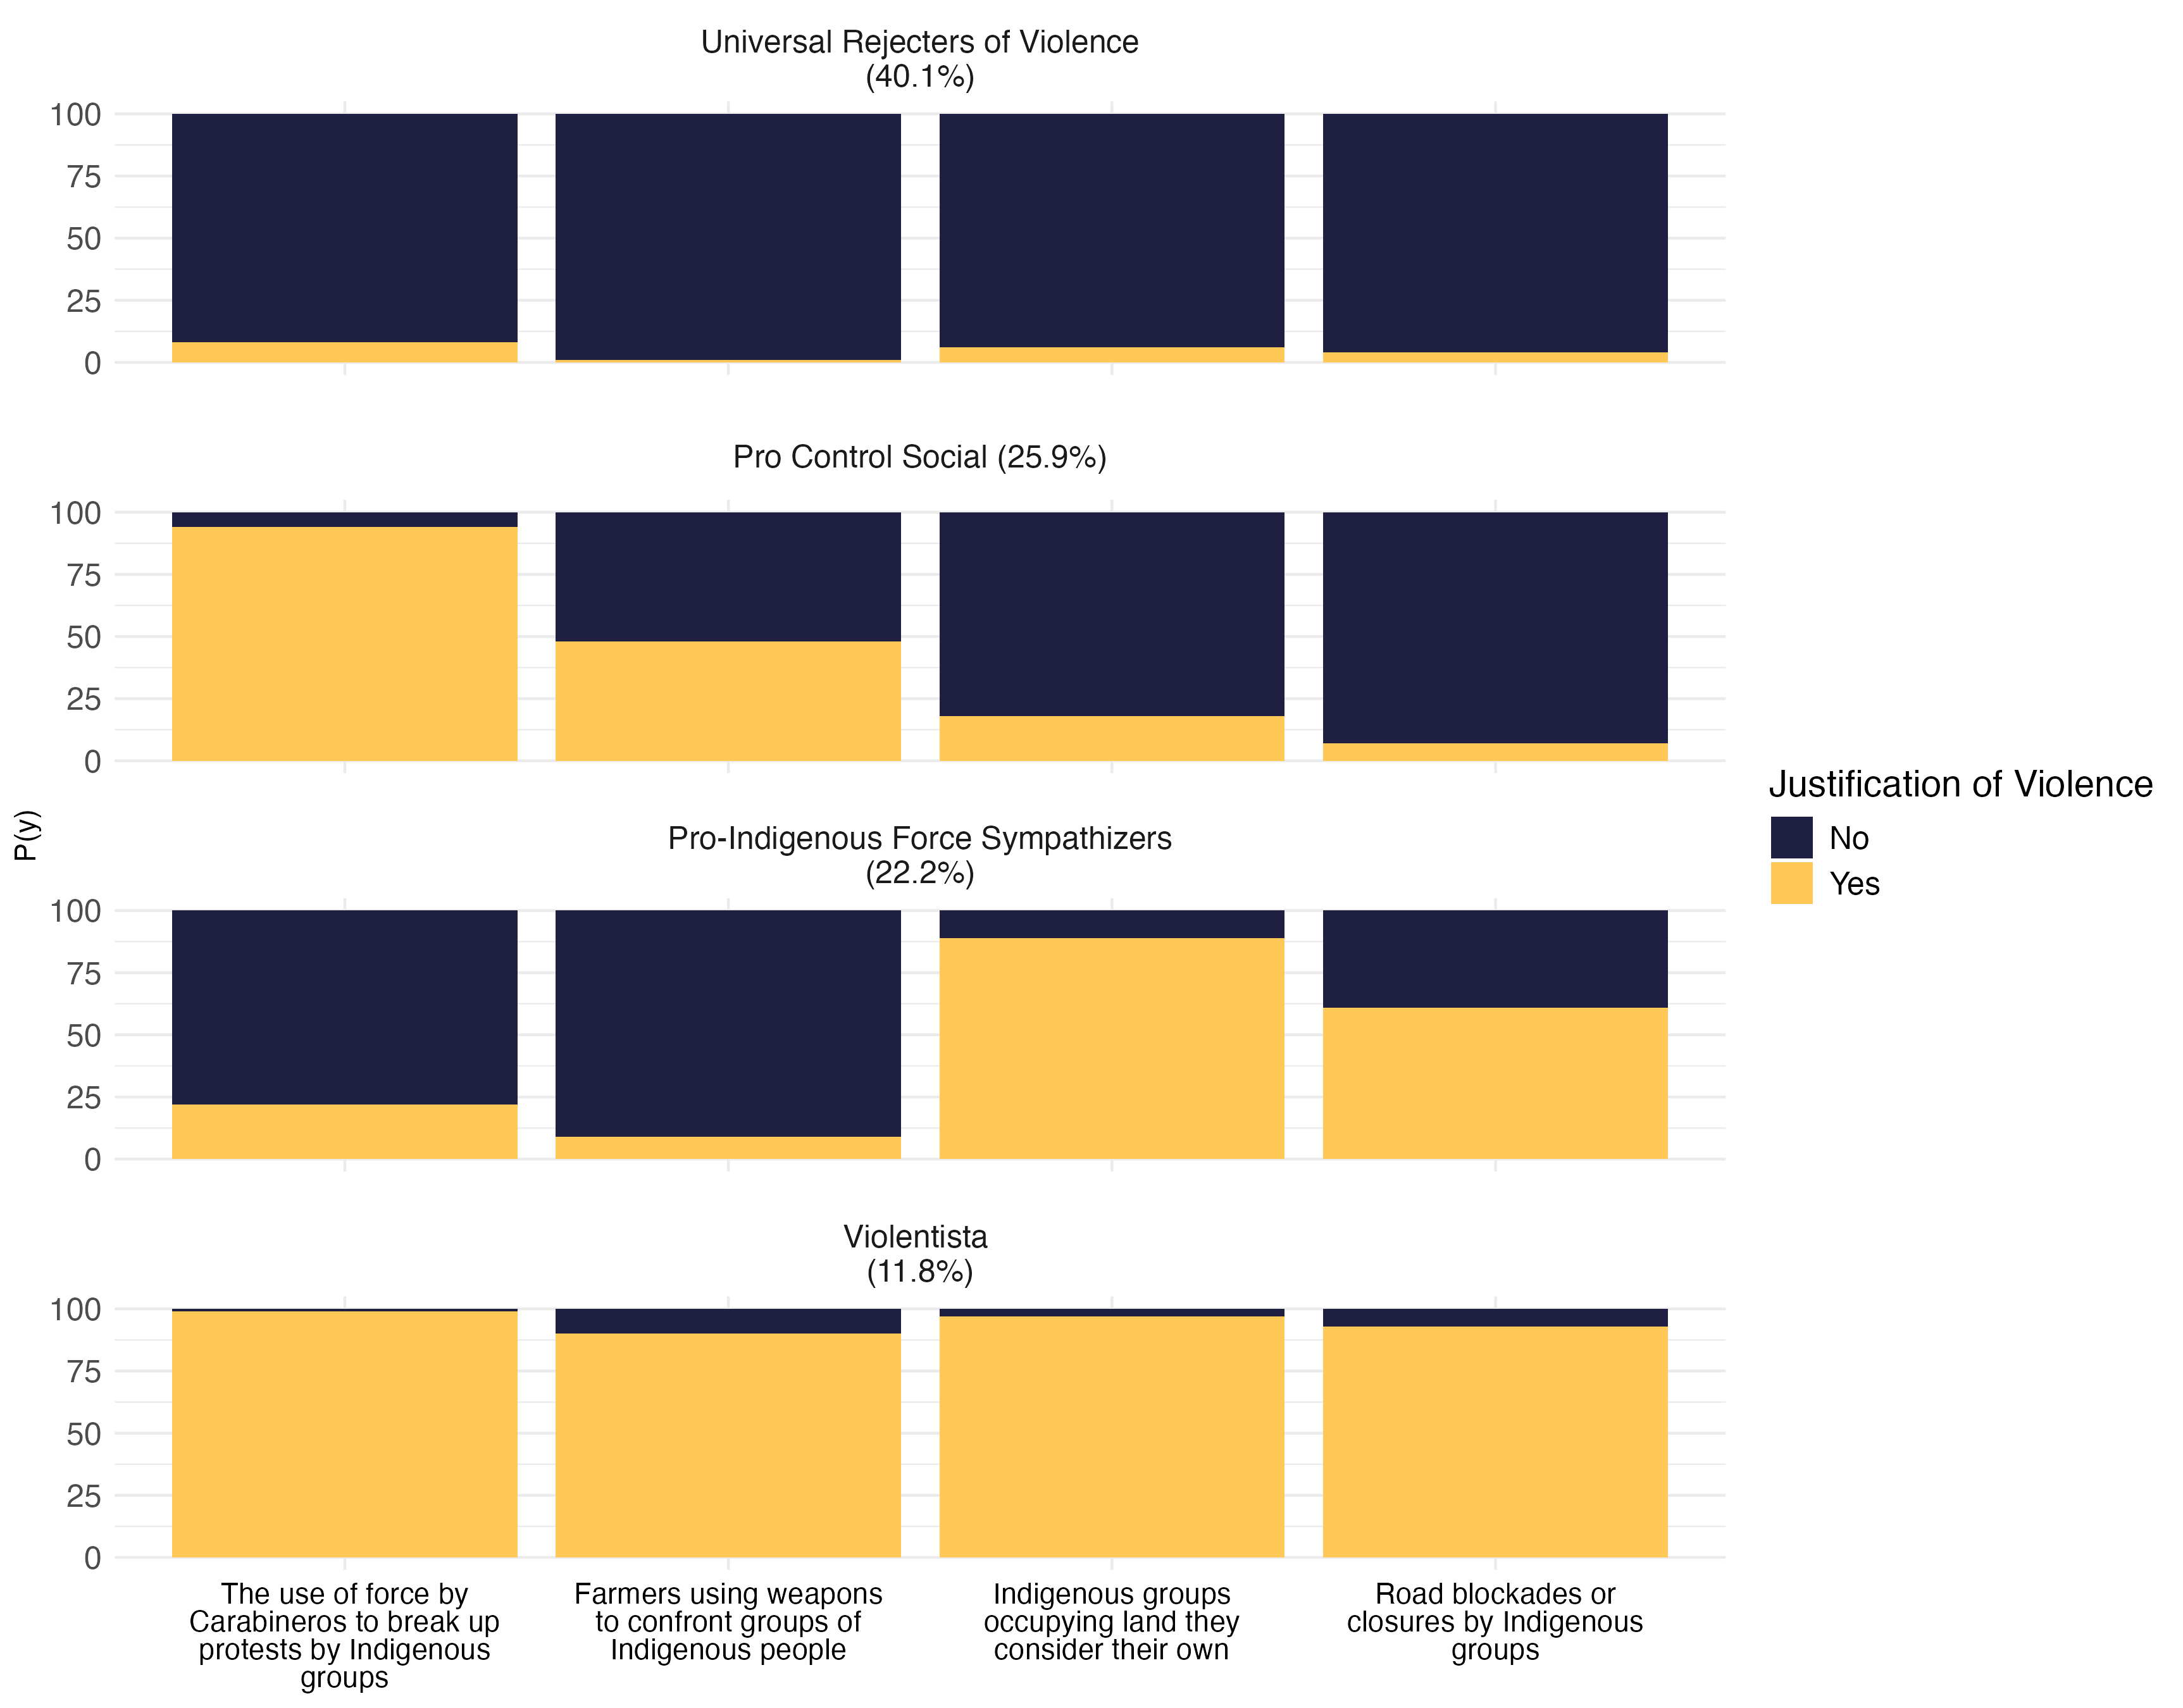
\includegraphics{images/p2-01.png}
\end{center}

\textbf{Resultado 2:} Probabilidad de pertenencia de las clases

\begin{table}

\caption{\label{tbl-predictores}}

\centering{

\caption*{
{\large \textbf{Predictores de pertenencia entre clases latentes}} \\ 
{\small Coeficientes y odds ratios (OR) del modelo de regresión multinomial}
} 
\fontsize{9.0pt}{10.8pt}\selectfont
\begin{tabular*}{\linewidth}{@{\extracolsep{\fill}}lllll}
\toprule
{\bfseries Variable} & Comparación & Coeficiente (IC 95\%) & OR (IC 95\%) & significativoicativo \\ 
\midrule\addlinespace[2.5pt]
confianza\_ppoo & Class 2 vs Class 1 & -0.339 [-0.574, -0.104] & 0.71 [0.56, 0.90] & {\cellcolor[HTML]{E6F4EA}{Sí (p < .05)}} \\ 
confianza\_ppoo & Class 3 vs Class 1 & -0.163 [-0.413, 0.086] & 0.85 [0.66, 1.09] & No \\ 
confianza\_ppoo & Class 4 vs Class 1 & -0.341 [-0.622, -0.059] & 0.71 [0.54, 0.94] & {\cellcolor[HTML]{E6F4EA}{Sí (p < .05)}} \\ 
conflicto\_estado & Class 2 vs Class 1 & 0.152 [-0.083, 0.387] & 1.16 [0.92, 1.47] & No \\ 
conflicto\_estado & Class 3 vs Class 1 & 0.468 [0.187, 0.748] & 1.60 [1.21, 2.11] & {\cellcolor[HTML]{E6F4EA}{Sí (p < .05)}} \\ 
conflicto\_estado & Class 4 vs Class 1 & 0.030 [-0.223, 0.283] & 1.03 [0.80, 1.33] & No \\ 
edad25\_34 & Class 2 vs Class 1 & 0.263 [-0.541, 1.066] & 1.30 [0.58, 2.90] & No \\ 
edad25\_34 & Class 3 vs Class 1 & -0.095 [-0.853, 0.663] & 0.91 [0.43, 1.94] & No \\ 
edad25\_34 & Class 4 vs Class 1 & -0.330 [-1.286, 0.625] & 0.72 [0.28, 1.87] & No \\ 
edad35\_44 & Class 2 vs Class 1 & 0.446 [-0.341, 1.232] & 1.56 [0.71, 3.43] & No \\ 
edad35\_44 & Class 3 vs Class 1 & -0.364 [-1.147, 0.418] & 0.69 [0.32, 1.52] & No \\ 
edad35\_44 & Class 4 vs Class 1 & 0.272 [-0.578, 1.121] & 1.31 [0.56, 3.07] & No \\ 
edad45\_54 & Class 2 vs Class 1 & -0.006 [-0.764, 0.753] & 0.99 [0.47, 2.12] & No \\ 
edad45\_54 & Class 3 vs Class 1 & -0.441 [-1.161, 0.280] & 0.64 [0.31, 1.32] & No \\ 
edad45\_54 & Class 4 vs Class 1 & -0.030 [-0.856, 0.796] & 0.97 [0.42, 2.22] & No \\ 
edad55\_64 & Class 2 vs Class 1 & -0.505 [-1.335, 0.325] & 0.60 [0.26, 1.38] & No \\ 
edad55\_64 & Class 3 vs Class 1 & -1.001 [-1.799, -0.203] & 0.37 [0.17, 0.82] & {\cellcolor[HTML]{E6F4EA}{Sí (p < .05)}} \\ 
edad55\_64 & Class 4 vs Class 1 & -0.547 [-1.399, 0.305] & 0.58 [0.25, 1.36] & No \\ 
edad65+ & Class 2 vs Class 1 & -0.210 [-1.016, 0.596] & 0.81 [0.36, 1.81] & No \\ 
edad65+ & Class 3 vs Class 1 & -0.791 [-1.640, 0.057] & 0.45 [0.19, 1.06] & No \\ 
edad65+ & Class 4 vs Class 1 & -0.263 [-1.125, 0.599] & 0.77 [0.32, 1.82] & No \\ 
frq\_contacto & Class 2 vs Class 1 & 0.124 [-0.068, 0.315] & 1.13 [0.93, 1.37] & No \\ 
frq\_contacto & Class 3 vs Class 1 & 0.084 [-0.102, 0.269] & 1.09 [0.90, 1.31] & No \\ 
frq\_contacto & Class 4 vs Class 1 & -0.205 [-0.427, 0.016] & 0.81 [0.65, 1.02] & No \\ 
id\_causa & Class 2 vs Class 1 & -0.569 [-0.781, -0.357] & 0.57 [0.46, 0.70] & {\cellcolor[HTML]{E6F4EA}{Sí (p < .05)}} \\ 
id\_causa & Class 3 vs Class 1 & 0.511 [0.263, 0.759] & 1.67 [1.30, 2.14] & {\cellcolor[HTML]{E6F4EA}{Sí (p < .05)}} \\ 
id\_causa & Class 4 vs Class 1 & 0.158 [-0.103, 0.418] & 1.17 [0.90, 1.52] & No \\ 
indiindi & Class 2 vs Class 1 & 0.447 [-0.009, 0.903] & 1.56 [0.99, 2.47] & No \\ 
indiindi & Class 3 vs Class 1 & 0.473 [0.013, 0.933] & 1.60 [1.01, 2.54] & {\cellcolor[HTML]{E6F4EA}{Sí (p < .05)}} \\ 
indiindi & Class 4 vs Class 1 & 0.586 [0.097, 1.075] & 1.80 [1.10, 2.93] & {\cellcolor[HTML]{E6F4EA}{Sí (p < .05)}} \\ 
intercept & Class 2 vs Class 1 & -0.794 [-2.467, 0.878] & 0.45 [0.08, 2.41] & No \\ 
intercept & Class 3 vs Class 1 & -3.563 [-5.552, -1.573] & 0.03 [0.00, 0.21] & {\cellcolor[HTML]{E6F4EA}{Sí (p < .05)}} \\ 
intercept & Class 4 vs Class 1 & -1.628 [-3.568, 0.312] & 0.20 [0.03, 1.37] & No \\ 
mujer1 & Class 2 vs Class 1 & -0.366 [-0.811, 0.079] & 0.69 [0.44, 1.08] & No \\ 
mujer1 & Class 3 vs Class 1 & -0.469 [-0.916, -0.022] & 0.63 [0.40, 0.98] & {\cellcolor[HTML]{E6F4EA}{Sí (p < .05)}} \\ 
mujer1 & Class 4 vs Class 1 & -0.327 [-0.834, 0.179] & 0.72 [0.43, 1.20] & No \\ 
procidimental\_ppoo & Class 2 vs Class 1 & 0.489 [0.258, 0.719] & 1.63 [1.29, 2.05] & {\cellcolor[HTML]{E6F4EA}{Sí (p < .05)}} \\ 
procidimental\_ppoo & Class 3 vs Class 1 & -0.293 [-0.535, -0.051] & 0.75 [0.59, 0.95] & {\cellcolor[HTML]{E6F4EA}{Sí (p < .05)}} \\ 
procidimental\_ppoo & Class 4 vs Class 1 & 0.873 [0.613, 1.133] & 2.39 [1.85, 3.11] & {\cellcolor[HTML]{E6F4EA}{Sí (p < .05)}} \\ 
urbano\_rural & Class 2 vs Class 1 & 0.798 [0.311, 1.284] & 2.22 [1.37, 3.61] & {\cellcolor[HTML]{E6F4EA}{Sí (p < .05)}} \\ 
urbano\_rural & Class 3 vs Class 1 & 0.609 [0.068, 1.151] & 1.84 [1.07, 3.16] & {\cellcolor[HTML]{E6F4EA}{Sí (p < .05)}} \\ 
urbano\_rural & Class 4 vs Class 1 & -0.733 [-1.444, -0.021] & 0.48 [0.24, 0.98] & {\cellcolor[HTML]{E6F4EA}{Sí (p < .05)}} \\ 
\bottomrule
\end{tabular*}

}

\end{table}%

\begin{center}
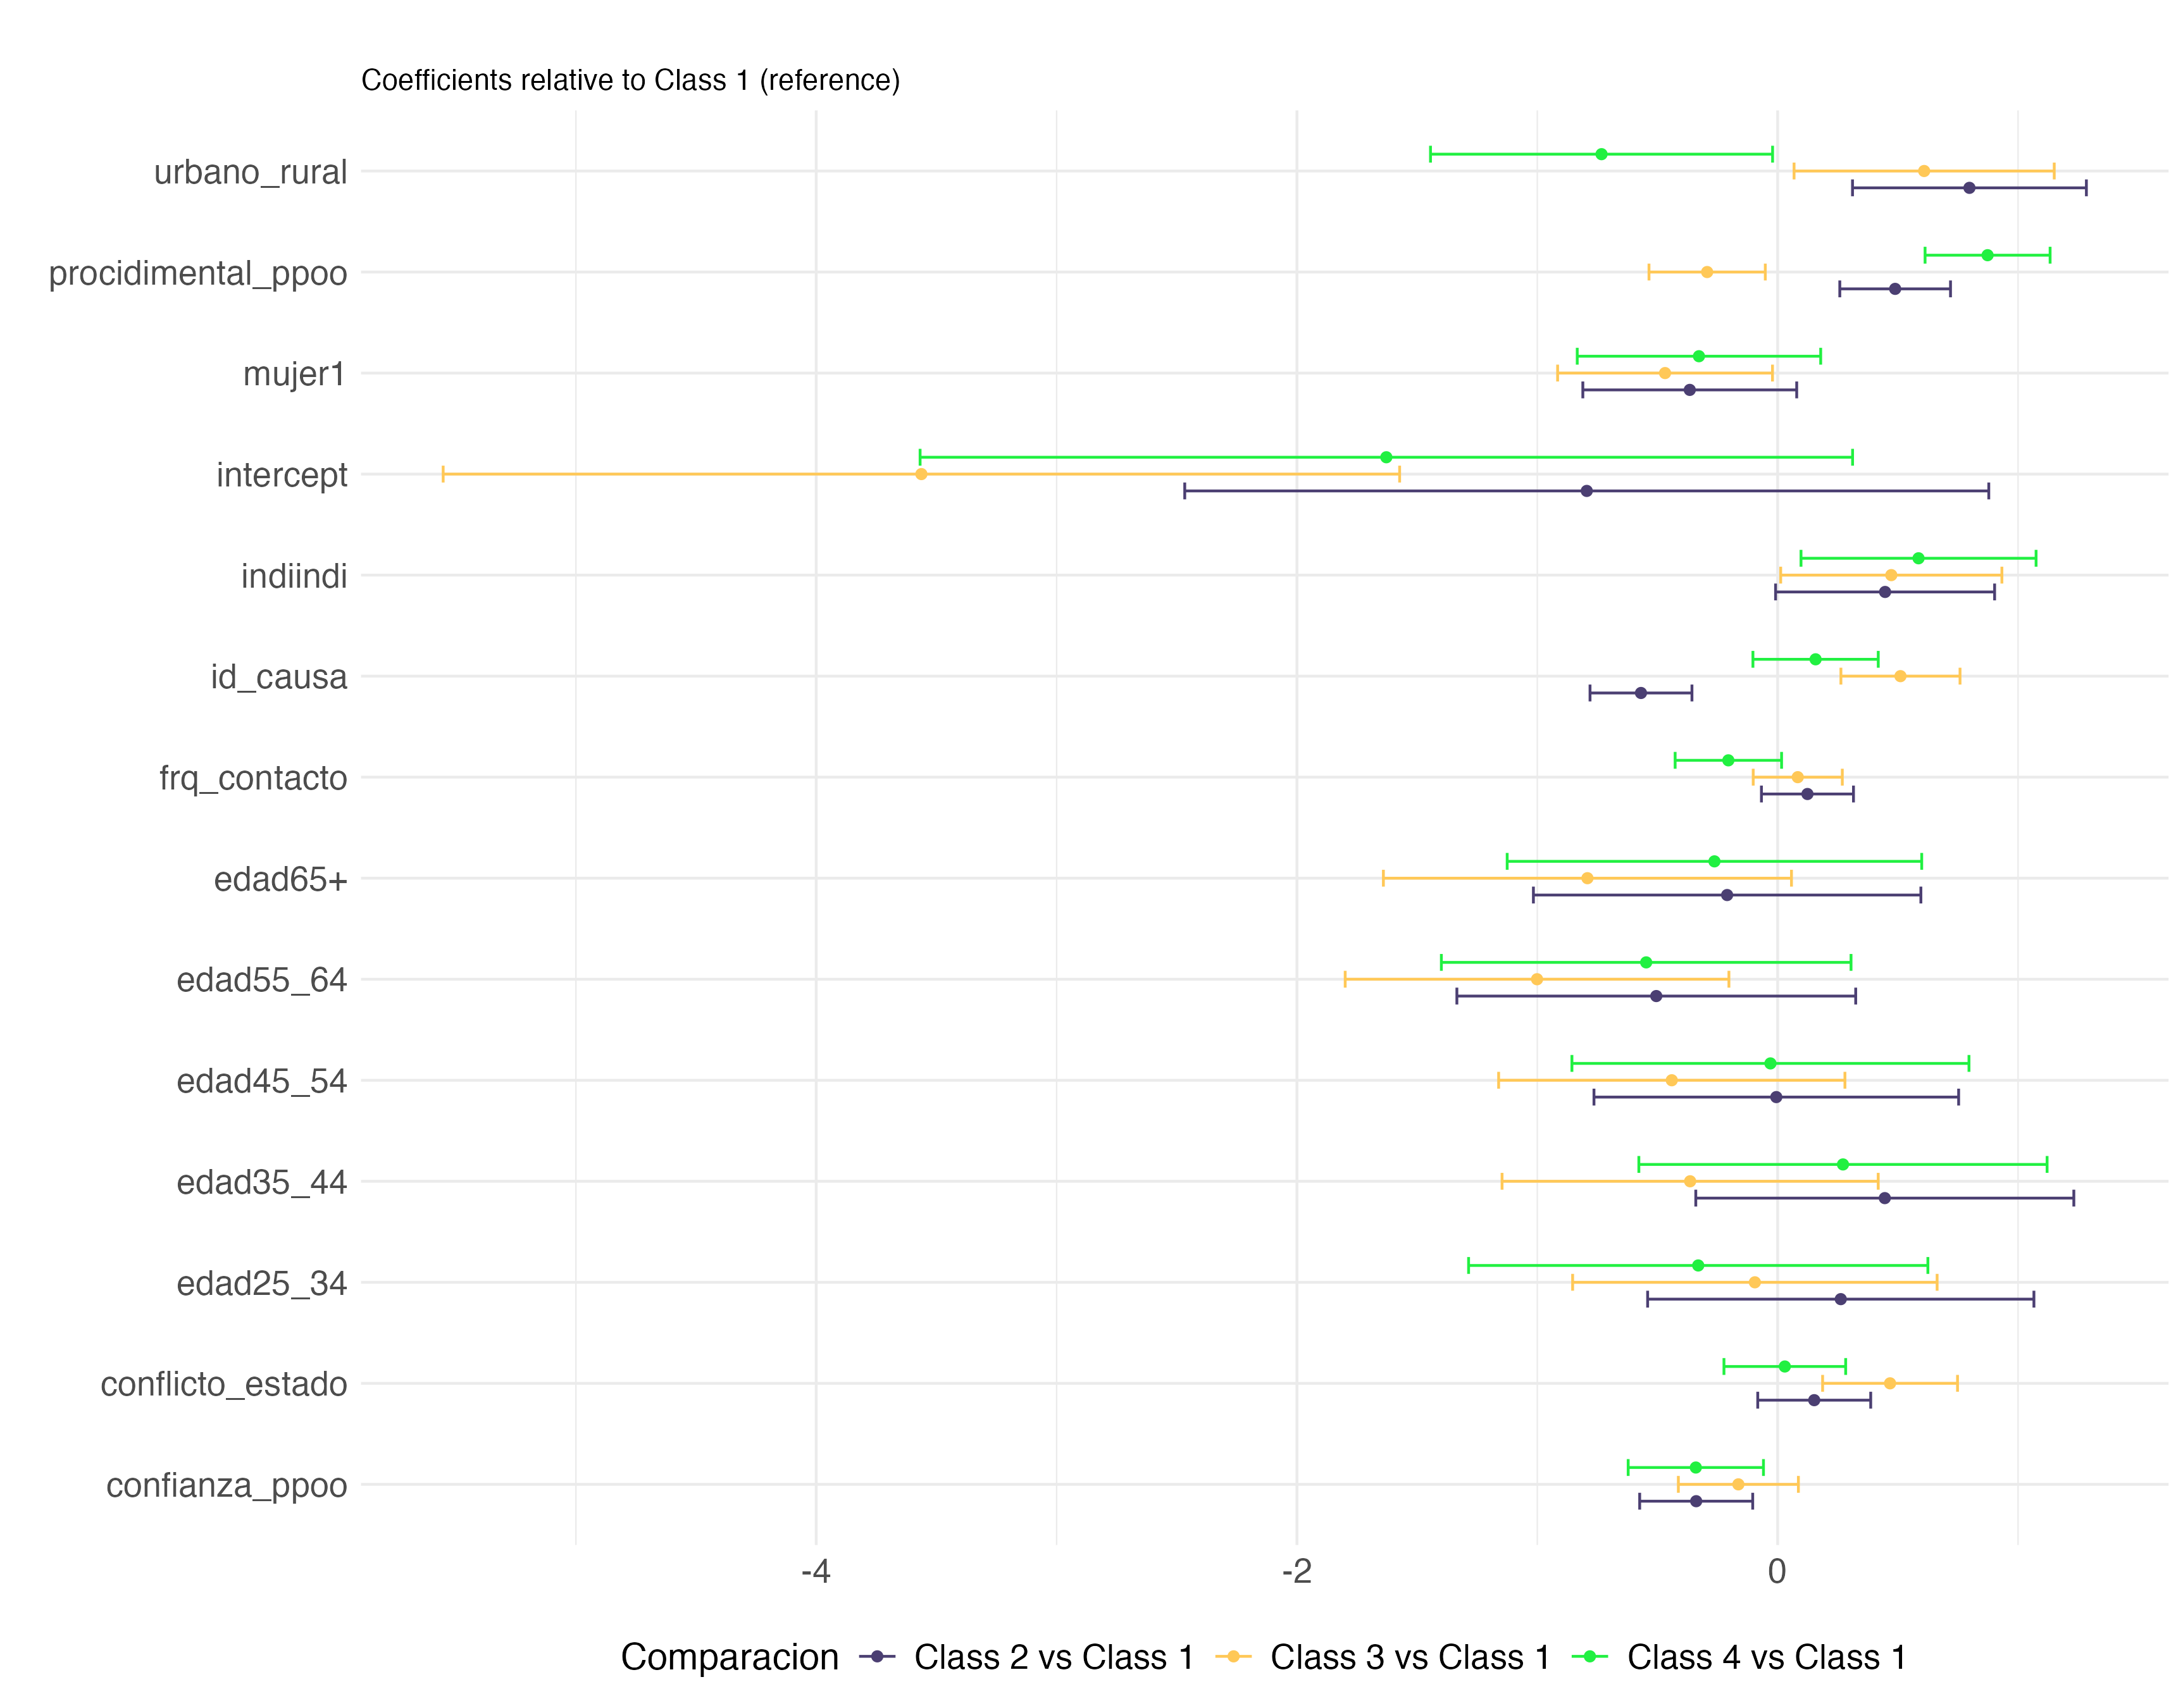
\includegraphics{images/p3.png}
\end{center}

\textbf{Resultado 3: Probabilidad de cambiarse de clase}

\begin{center}
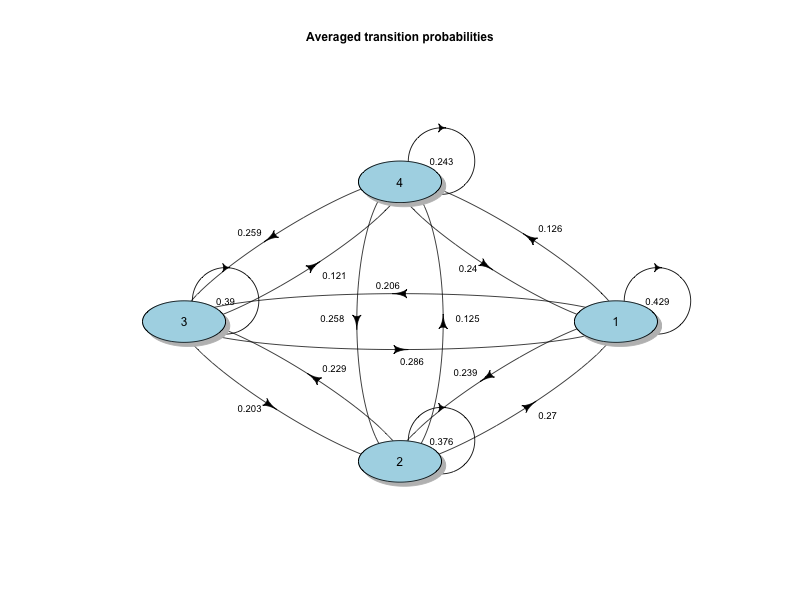
\includegraphics{images/transition_modelo_4c.png}
\end{center}

\begin{table}

\caption{\label{tbl-transiciones}}

\centering{

\caption*{
{\large \textbf{Odds ratio de transición desde la Clase 1}} \\ 
{\small Probabilidad relativa de pasar a las Clases 2, 3 y 4 (ref. = Clase 1)}
} 
\fontsize{9.0pt}{10.8pt}\selectfont
\begin{tabular*}{\linewidth}{@{\extracolsep{\fill}}lrrrrrr}
\toprule
 & \multicolumn{2}{c}{Transición a Clase 2} & \multicolumn{2}{c}{Transición a Clase 3} & \multicolumn{2}{c}{Transición a Clase 4} \\ 
\cmidrule(lr){2-3} \cmidrule(lr){4-5} \cmidrule(lr){6-7}
{\bfseries Variable} & OR Clase 2 vs 1 & p & OR Clase 3 vs 1 & p & OR Clase 4 vs 1 & p \\ 
\midrule\addlinespace[2.5pt]
Frecuencia de contacto con pueblos originarios & 1.09 & 0.423 & 1.18 & 0.122 & 0.83 & 0.100 \\ 
Confianza en pueblos originarios & {\cellcolor[HTML]{E6F4EA}{0.78}} & 0.028 & 0.95 & 0.690 & {\cellcolor[HTML]{E6F4EA}{0.67}} & 0.002 \\ 
Percepción conflicto Estado–Pueblos Originarios & 1.13 & 0.260 & {\cellcolor[HTML]{E6F4EA}{1.30}} & 0.047 & {\cellcolor[HTML]{E6F4EA}{1.67}} & 0.001 \\ 
Justicia procedimental hacia pueblos indígenas & {\cellcolor[HTML]{E6F4EA}{2.06}} & 0.000 & 0.81 & 0.065 & {\cellcolor[HTML]{E6F4EA}{1.91}} & 0.000 \\ 
Identificación con la causa indígena & {\cellcolor[HTML]{E6F4EA}{0.78}} & 0.016 & {\cellcolor[HTML]{E6F4EA}{1.49}} & 0.002 & 1.23 & 0.119 \\ 
Edad 25–34 años & 0.48 & 0.215 & 1.61 & 0.491 & 0.35 & 0.166 \\ 
Edad 35–44 años & 0.88 & 0.823 & 2.01 & 0.324 & 1.12 & 0.877 \\ 
Edad 45–54 años & 1.90 & 0.259 & 3.00 & 0.115 & 0.93 & 0.921 \\ 
Edad 55–64 años & 0.94 & 0.908 & 1.38 & 0.646 & 0.78 & 0.731 \\ 
Edad 65 o más & 1.20 & 0.744 & 1.43 & 0.605 & 1.23 & 0.770 \\ 
Identidad indígena (1 = sí, 0 = no) & 0.88 & 0.592 & 1.08 & 0.739 & 1.76 & 0.056 \\ 
intercept & 0.31 & 0.217 & {\cellcolor[HTML]{E6F4EA}{0.05}} & 0.007 & {\cellcolor[HTML]{E6F4EA}{0.01}} & 0.000 \\ 
Mujer (1 = mujer, 0 = hombre) & 1.10 & 0.686 & 1.14 & 0.580 & 1.46 & 0.170 \\ 
Zona urbana (1 = urbano, 0 = rural) & 0.63 & 0.113 & 0.51 & 0.052 & 1.59 & 0.107 \\ 
\bottomrule
\end{tabular*}

}

\end{table}%

\begin{center}
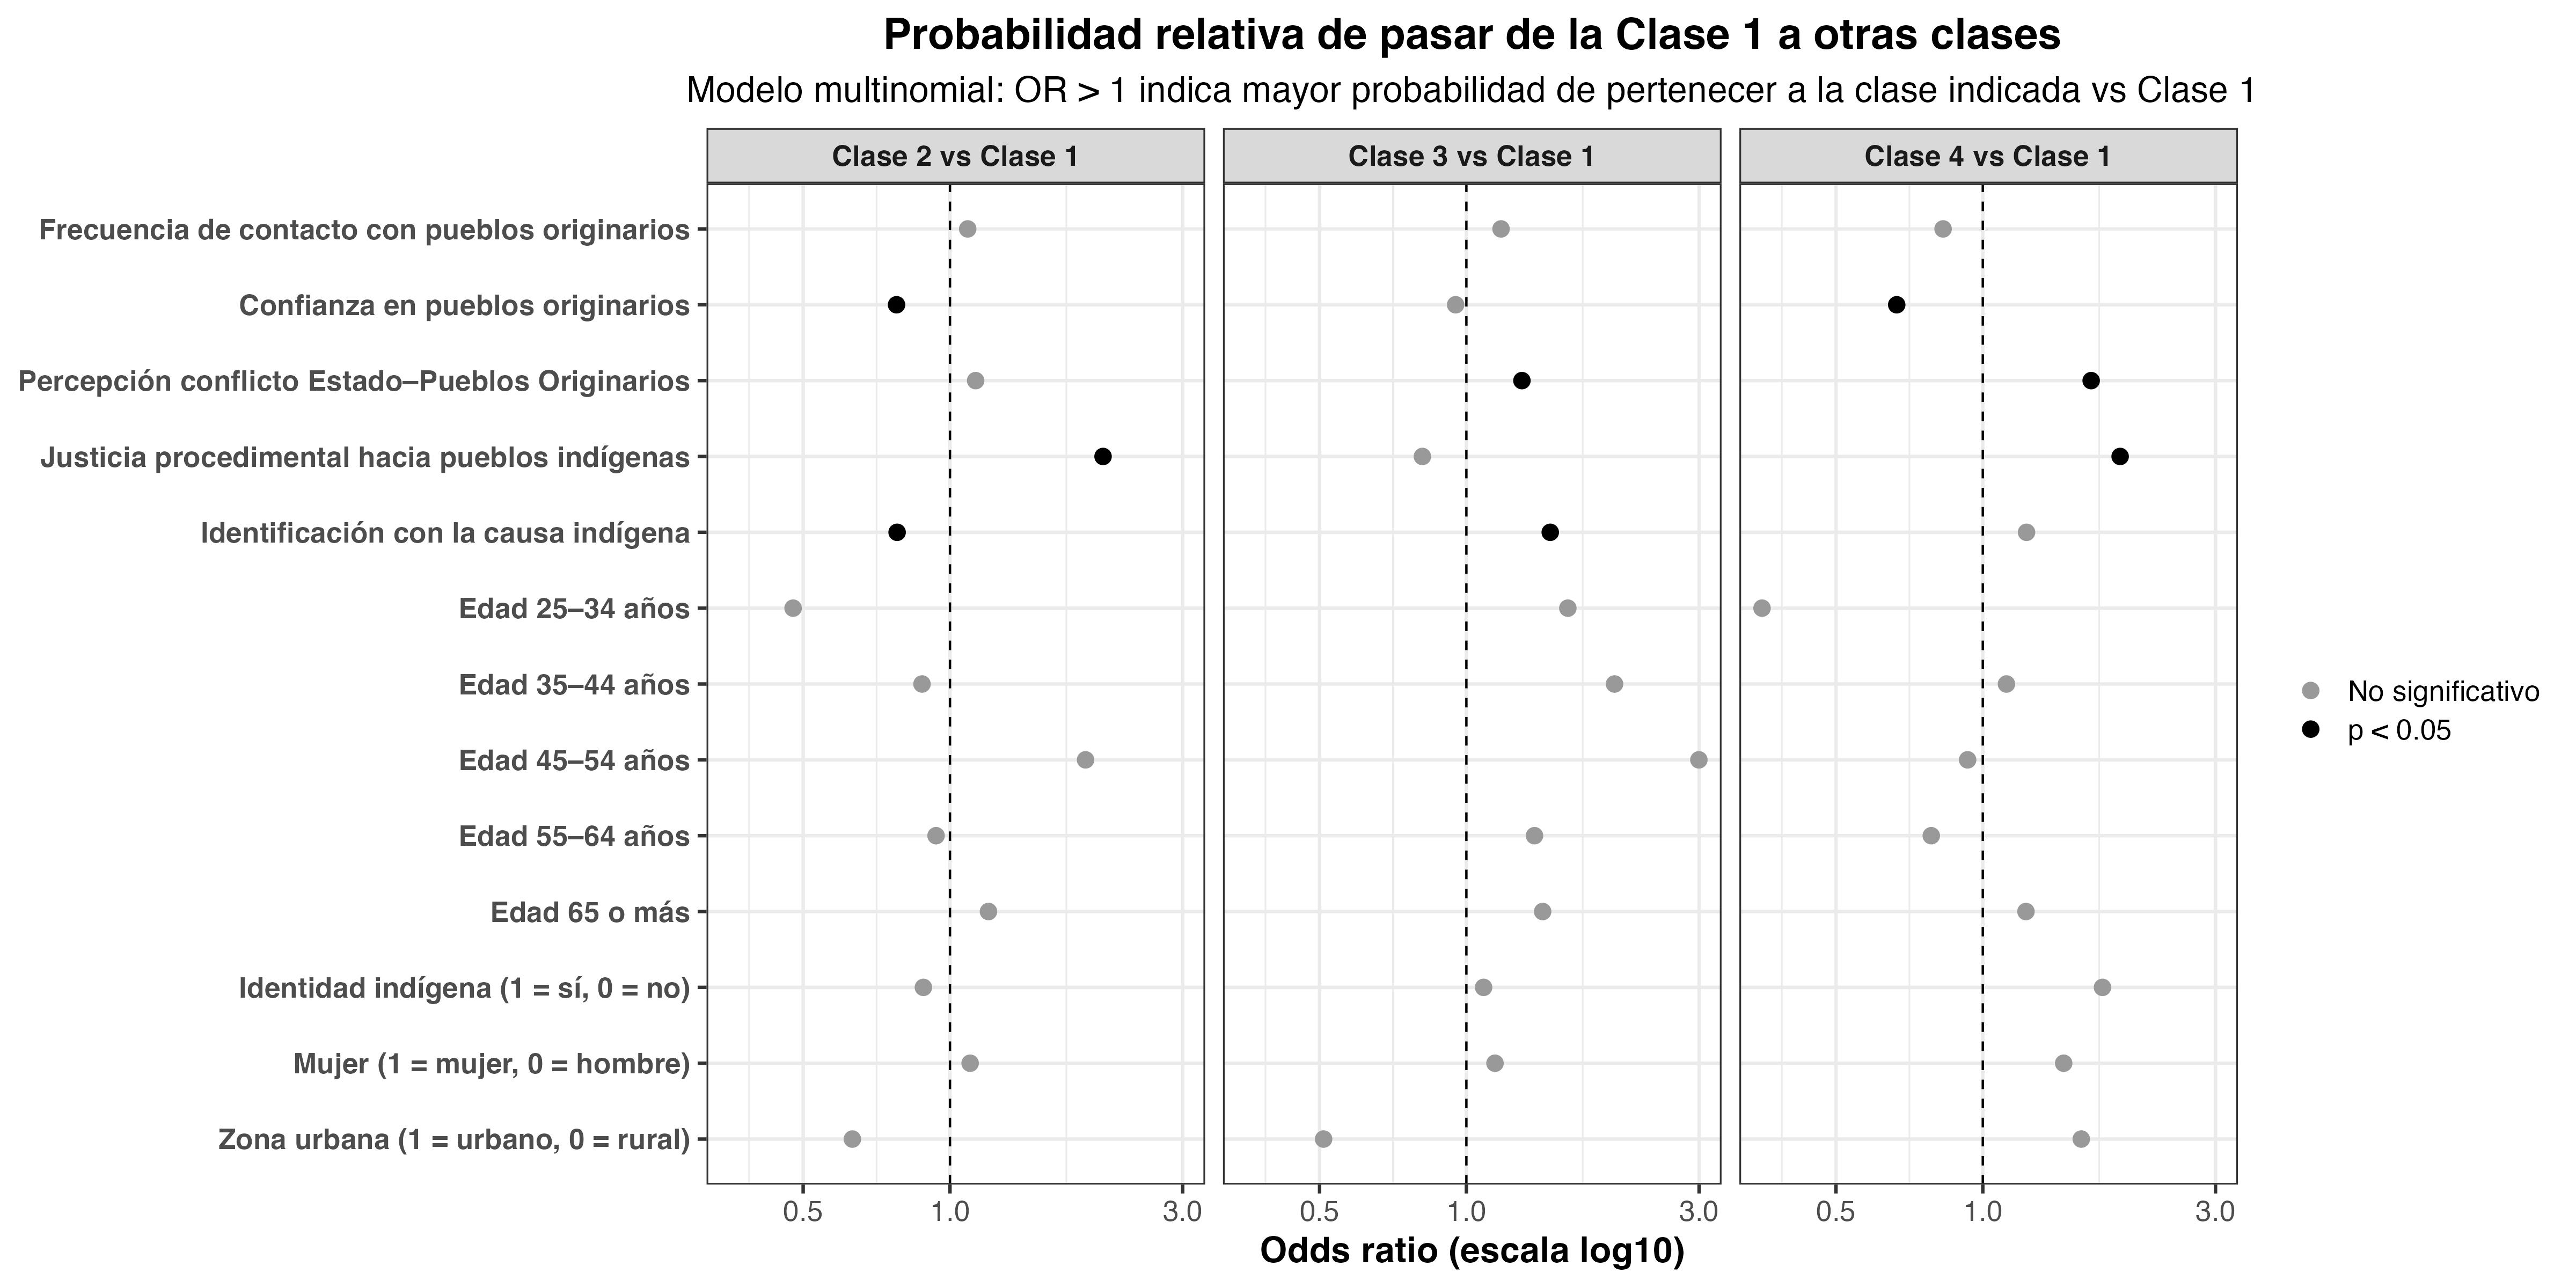
\includegraphics{images/probabilidad_respuesta1-01.jpg}
\end{center}

\section{5. Discusión}\label{discusiuxf3n}

(Por completar: implicancias teóricas, políticas, contribuciones al
estudio del conflicto indígena.)

\section{6. Conclusión}\label{conclusiuxf3n}

(Por completar.)

\section{Referencias}\label{referencias}

(Agregar luego con pandoc csl.)




\end{document}
